\documentclass[12pt,a4paper,twoside]{article}
\usepackage{fancyhdr,graphicx,latexsym}

\setlength{\parindent}{0cm}
\setlength{\parskip}{2ex plus1ex minus 0.5ex}

\addtolength{\evensidemargin}{-2.5cm}
\addtolength{\oddsidemargin}{-0.5cm}
\addtolength{\textwidth}{3cm}

\addtolength{\headheight}{0.2cm}
\addtolength{\topmargin}{-1cm}
\addtolength{\textheight}{2.5cm}

\renewcommand{\_}{\texttt{\symbol{95}}}
\addtolength{\fboxsep}{0.1cm}
\newcommand{\param}[1]{\textit{\textrm{\textmd{#1}}}}
\newcommand{\codebar}{\rule{\textwidth}{0.3mm}}
% \newcommand{\spc}{\hspace{0.5mm}$\sqcup$\hspace{0.6mm}}
\newcommand{\spc}{\hspace{0.5mm}$\Box$\hspace{0.5mm}}
\newcommand{\todo}[1]{\textbf{TODO: #1}}

\renewcommand{\textfraction}{0.05}
\renewcommand{\topfraction}{0.85}
\renewcommand{\bottomfraction}{0.65}
\renewcommand{\floatpagefraction}{0.60}

\newlength{\codelen}
\newcommand{\code}[1]
{\begin{center}\fbox{\parbox{16cm}{\texttt{#1}}}\end{center}}

\fancyhead{}
\fancyhead[RO,LE]{\thepage}
\fancyhead[LO,RE]{PIRATES Protocol}
\fancyfoot{}
\pagestyle{empty}

\newenvironment{bulletlist}
{
	\begin{itemize}
	\setlength{\itemsep}{0ex}
	\setlength{\parsep}{0ex}
}
{
	\end{itemize}
}

\newenvironment{alphalist}
{
	\begin{enumerate}
	\setlength{\itemsep}{0ex}
	\setlength{\parsep}{0ex}
	\renewcommand{\labelenumi}{(\alph{enumi})}
}
{
	\end{enumerate}
}

\newenvironment{numericlist}
{
	\begin{enumerate}
	\setlength{\itemsep}{0ex}
	\setlength{\parsep}{0ex}
}
{
	\end{enumerate}
}

\begin{document}

% \sfseries
\centerline{\textbf{\LARGE PIRATES Protocol}}
\begin{center} \large
David Ingram\\
TIME-EACM Project\\
University of Cambridge Computer Lab\\
12th August 2009\\
\end{center}

{ \parskip 1mm plus 1pt \tableofcontents }
\pagestyle{fancy}

\newpage
\section{Introduction}
\label{intro}

This document describes the PIRATES \textbf{protocol version 8}.
The information here is only of use to internal PIRATES developers;
ordinary developers writing PIRATES components do not need to know
how the protocol works.

Figure \ref{dataseq} shows the possible message sequences used
on the data connections between library and wrapper, and also from
wrapper to wrapper between two components.

\begin{figure}[h]
\centering
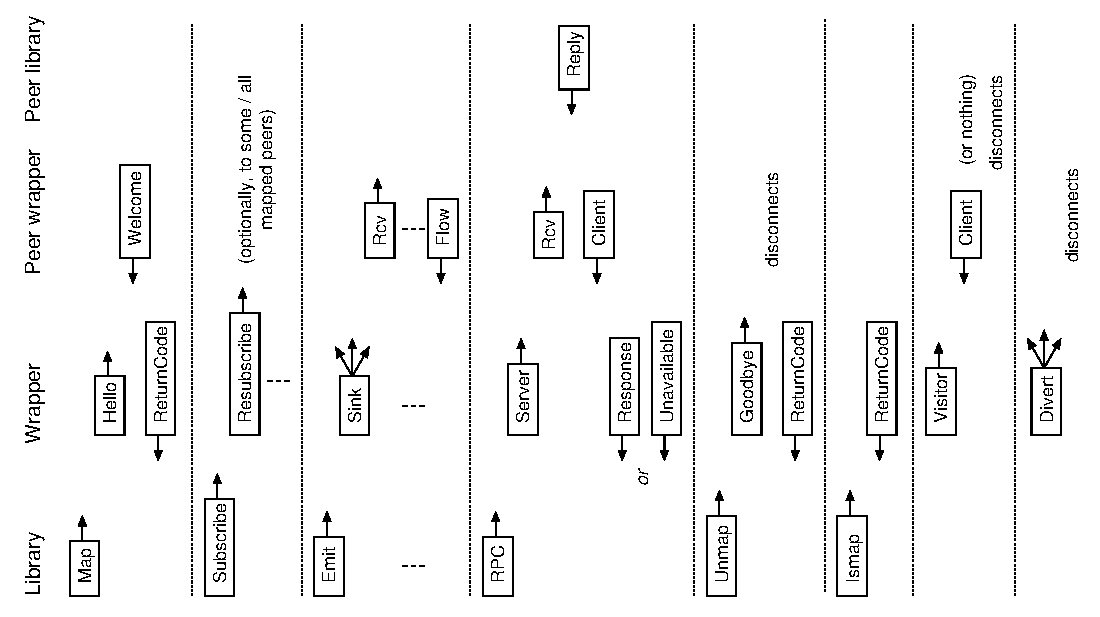
\includegraphics[scale=0.9,angle=-90]{diagrams/dataseq.eps}
\caption{Endpoint data connection message sequences}
\label{dataseq}
\end{figure}
\newpage

\subsection{Message headers}

The first 10 bytes of any message is in a fixed format,
regardless of the message type (including internal library to
wrapper communications).

\begin{tabular}{|ll|}
\hline
magic string       & 4 bytes\\
protocol version   & 1 byte\\
message length     & 4 bytes\\
message type       & 1 byte\\
\hline
\end{tabular}

Headers start with the magic string \texttt{sBuS}.
This is followed by a one byte protocol version and then
the total message length stored as a four byte integer.
Finally there is a one byte message type identifier
which contains a value from the MessageType enum.

The header format is guaranteed never to change before the end of
the message type field.
A fixed read of the first 10 bytes will therefore discover
the protocol version, message length and type (and nothing else).

\section{Component to Component protocol}
\label{cpt-cpt}

A separate TCP
connection is used for every map. Even if several endpoints are mapped
between the textit{same} pair of components, they will have several independent
connections.

Endpoints may of course be simultaneously mapped to more than one other
component, in which case there will be several TCP connections with
different destinations managed by a single endpoint.

The message types used for
component to component communication
are as follows:

\begin{verbatim}
enum MessageType
{
   // Component to component:
	
   MessageHello, MessageWelcome,              // Remote connection setup
   MessageSink, MessageServer, MessageClient, // Remote data transfer
   MessageFlow,                // Flow control, sent from sink to source
   MessageGoodbye, MessageResubscribe, MessageDivert, // Out-of-band messages
   MessageVisitor,                            // Disposable connections
   ...
}
\end{verbatim}

\subsection{Connection setup}

Connection setup between two components consists of a simple two message
handshake (one in each direction). Either party may open the connection,
so sources can connect to sinks and vice versa (it is even possible
for servers to connect to clients, although it would certainly be
more normal for a client to connect to a server). The connection setup
protocol occurs when a \textit{mapping} is made using the API.

\begin{bulletlist}
\item Initial component opens a TCP connection to the target component's
	listening port
\item Incoming connection is accepted by the target component
\item Initial component sends a MessageHello, specifying their name,
	the component name they think they have connected to, the endpoint
	they want, the API (hash codes) they are expecting it to use,
	and (if connecting to a source) subscription details
\item Target component replies with a MessageWelcome. This includes,
	amongst other things,
	a one-byte acceptance code, which takes one of the following values:\\
	\verb^AcceptOK^, \verb^AcceptWrongCpt^ (component name mismatch),
	\verb^AcceptNoEndpoint^ (no such endpoint),
	\verb^AcceptWrongType^ (endpoint type is incorrect),
	\verb^AcceptNotCompatible^ (endpoint API hash incompatible),
	\verb^AcceptNoAccess^ (lack of privilege), \verb^AcceptProtocol^\\
	\verb^Error^ or \verb^AcceptAlreadyMapped^.
\item If the acceptance code sent by the target component was
	\textit{not} \verb^AcceptOK^,
	it now closes the connection. Otherwise the connection has been made,
	and the file
	descriptors are added by both the initial and target components to
	the list ssociated with their relevant endpoint.
\end{bulletlist}

Hello message:

\begin{tabular}{|ll|}
\hline
standard header    & 10 bytes\\
\multicolumn{2}{|c|}{type = MessageHello}\\
\hline
sending component name    & count, string\\
sending component address & count, string\\
sending instance name     & count, string\\
from endpoint name        & count, string\\
from endpoint ID          & count\\
target component name     & count, string\\
endpoint required         & count, string\\
endpoint ID required      & count\\
target endpoint type      & 1 byte\\
subscription expression   & count, string\\
subscription topic        & count, string\\
message hash              & 6 bytes\\
response hash             & 6 bytes\\
\hline
\end{tabular}\\

In the message body, note that all string fields are preceded by a count
of their length, and are not NULL terminated.

The response hash field will contain the ``inapplicable'' hash code
(\verb^EEEEEEEEEEEE^) if the endpoint
type is source or sink. The two subscription fields are only used
when connecting to source endpoints (otherwise they should be
transmitted as empty strings, and will be ignored).

The target replies with its identity in a welcome message:

\begin{tabular}{|ll|}
\hline
standard header    & 10 bytes\\
\multicolumn{2}{|c|}{type = MessageWelcome}\\
\hline
acceptance code    & 1 byte\\
component name     & count, string\\
instance name      & count, string\\
endpoint name      & count, string\\
component address  & count, string\\
subscription expression & count, string\\
subscription topic      & count, string\\
message polymorphic     & 1 byte (0 or 1)\\
reply polymorphic       & 1 byte (0 or 1)\\
\hline
\end{tabular}\\

The two subscription fields in the welcome message are only used if the
component sending the welcome message is of type sink (otherwise they
should be sent as empty strings).

The polymorphism fields are flags indicating whether the component
sending the welcome is polymorphic for messages and/or replies
on this connection. The actual hash codes are not returned, since
if it is not polymorphic then an acceptance code of \verb^AcceptOK^
implies they match those sent in the MessageHello.

\subsection{Normal (data) message format}

This is represented by the \verb^scomm^ structure internally.

\begin{tabular}{|ll|}
\hline
standard header    & 10 bytes\\
\multicolumn{2}{|c|}{type = MessageSink $|$ MessageServer $|$ MessageClient}\\
\hline
sending component name  & count, string\\
sending endpoint name  & count, string\\
target component name   & count, string\\
target endpoint name    & count, string\\
topic              & count, string\\
session seq ID     & count\\
source seq ID      & count\\
api hash           & 6 bytes\\
DATA               & variable length\\
\hline
\end{tabular}\\

This message format is used for normal data communications between
components. The message type is named after the type of the target
endpoint (e.g. MessageSink if it is being sent to a sink endpoint).
There is no such type as MessageSource, because in-band messages are
never sent \textit{to} sources.

The target component name should match the component which is
receiving the message, unless it is the demux component.

The session seq ID allows RPC replies to be matched to queries,
and source seq ID helps with stream migration.

The topic field is only used for MessageSink, and provides the
topic specified when the message was emitted (if any).

\subsection{Flow control}

This message type is sent from sink to source endpoints only.

\begin{tabular}{|ll|}
\hline
standard header    & 10 bytes\\
\multicolumn{2}{|c|}{type = MessageFlow}\\
\hline
sending component name  & count, string\\
sending endpoint name   & count, string\\
target component name   & count, string\\
target endpoint name    & count, string\\
window                  & count\\
\hline
\end{tabular}\\

The window field provides information about the sequence numbers the
source may transmit before it must pause and await further flow
control messages from the sink. Flow control is therefore proactive
(based on prior authorisation to send) rather than reactive.

Parameters: \verb^OutputBufferSize, WindowSize, MaxDelay (ms)^

\subsection{Out of band messages}

These are control messages which are consumed by the wrapper, and not
passed up to the component. They are specified by message types.
They are sent on data connections and may occur anywhere that a
MessageSink, MessageServer or MessageClient could, as well as being
sent to sources (which do not normally receive any messages at all).

\subsubsection{Connection closure}

\begin{tabular}{|ll|}
\hline
standard header    & 10 bytes\\
\multicolumn{2}{|c|}{type = MessageGoodbye}\\
\hline
sending component name  & count, string\\
sending endpoint name   & count, string\\
target component name   & count, string\\
target endpoint name    & count, string\\
\hline
\end{tabular}\\

A message type of MessageGoodbye indicates a deliberate close of the connection
(if this message is not sent before closing the connection, the other
side may assume something has failed and try to reconnect it).

\subsubsection{Resubscribe}

\begin{tabular}{|ll|}
\hline
standard header    & 10 bytes\\
\multicolumn{2}{|c|}{type = MessageResubscribe}\\
\hline
sending component name  & count, string\\
sending endpoint name   & count, string\\
target component name   & count, string\\
target endpoint name    & count, string\\
subscription       & count, string\\
topic              & count, string\\
\hline
\end{tabular}\\

\subsubsection{Divert}

\begin{tabular}{|ll|}
\hline
standard header    & 10 bytes\\
\multicolumn{2}{|c|}{type = MessageDivert}\\
\hline
sending component name  & count, string\\
sending endpoint name   & count, string\\
target component name   & count, string\\
target endpoint name    & count, string\\
new component name      & count, string\\
new endpoint name       & count, string\\
\hline
\end{tabular}\\

%\subsubsection{Future out of band messages}
%
%All of the messages in this section are unimplemented at present.
%
%\verb^error^, \verb^exception^, \verb^denied^,
%\verb^transfer^, \verb^freeze^ and \verb^unfreeze^.
%
%\verb^error^ contains an error code/reason in the message body.
%It is returned if the component name does not match the one
%requested, or if the request if invalid.
%
%\verb^denied^ indicates an access control refusal.
%
%\verb^exception^ is caused by an application-level exception return
%value. Instead of a normally formatted reply the body contains an
%explanatory string.
%
%\verb^transfer^, \verb^freeze^ and \verb^unfreeze^
%are for dynamic reconfiguration.
%
%\textbf{Error sequences}
%
%Currently the action taken in any of these cases is to log the error and
%terminate immediately:
%
%\begin{bulletlist}
%\item Bad magic number
%\item Garbled header
%\item Incorrect sequence number
%\item Unexpected message
%\item Corrupt XML
%\item Illegal data
%\end{bulletlist}

\subsection{Disposable connections}

These are only used internally by the wrapper when communicating
with other wrappers; they are not exposed to the API. Uses include
calling \verb^lookup_schema^ to fetch the schema needed to decipher
a received message of an unknown type, calling \verb^lookup_cpt^
on the RDC during mapping by constraints, and \verb^register_cpt^
to register with the RDC.

These connections allow a single RPC to be made (or message to be
sent), after which the connection is always closed. They are
lighter weight than ordinary connections, because the calling side
does not use an explicit endpoint and the transient connection therefore
does not appear in the component's status. This is useful for the
wrapper as it must sometimes do several lookups at once and there is
no way to dynamically create extra formal client endpoints to handle this.

Another advantage is that there is no handshake: the Hello message is combined
with the RPC query and the Welcome message is combined with the reply. This
simplifies state management inside the wrapper when it is waiting for a lookup
to return before it can proceed with some other task (because the wrapper is
non-blocking, it must do this asynchronously and keep track of which phase of
an action it was last in, which would be a lot more complex for endpoints that
have to be mapped before use).

The initial message sent over a disposable connection is of type
Visitor, and the reply, if there is one, of type Client.
The side which initiates (effectively, maps) a disposable connection
must be the side making an RPC or sending a message.

\begin{tabular}{|ll|}
\hline
standard header    & 10 bytes\\
\multicolumn{2}{|c|}{type = MessageVisitor}\\
\hline
sending component name  & count, string\\
from pseudo-endpoint UID          & count\\
target component name   & count, string\\
endpoint required  & count, string\\
target endpoint type    & 1 byte (Sink or Server)\\
message hash       & 6 bytes\\
expected response hash      & 6 bytes\\
DATA               & variable length\\
\hline
\end{tabular}\\

\section{Library to Wrapper Protocol}
\label{lib-wrapper}

The message types used for library to wrapper communication inside
a component are as follows:

\begin{verbatim}
enum MessageType
{
   ...
	
   // Library to wrapper:
   
   MessageAddEndpoint, MessageStart,       // Bootstrap pipe setup
   MessageStop,                            // Bootstrap pipe runtime/close
   MessageRunning,                         // Reply on bootstrap pipe
   MessageGetStatus, MessageStatus,        // Bootstrap pipe runtime
   MessageGetSchema, MessageSchema,        // Bootstrap pipe runtime
   MessageDeclare, MessageHash,            // Bootstrap pipe runtime
   MessageMap, MessageUnmap, MessageIsmap, // Mapping control messages
   MessageReturnCode,                      // Mapping control reply
   MessageSubscribe,                       // Endpoint control message
   MessageEmit, MessageRPC, MessageReply,  // Library to wrapper data
   MessageRcv, MessageResponse, MessageUnavailable // Wrapper to library data
};
\end{verbatim}

Figure \ref{controlseq} shows the message sequences
used on the \textit{bootstrap connection} between
the library and the wrapper. See Figure \ref{dataseq} from
Section \ref{intro} for the message sequences
used on the data connections between library and wrapper.

\begin{figure}[h]
\centering
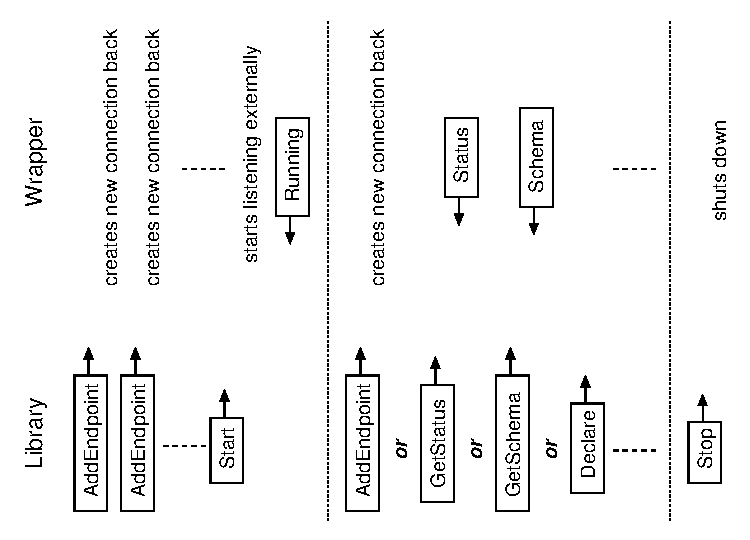
\includegraphics[scale=1.0,angle=-90]{diagrams/controlseq.eps}
\caption{Master bootstrap connection message sequence}
\label{controlseq}
\end{figure}

\subsection{Bootstrap wrapper initialisation}

The wrapper is called with a command-line argument specifying the
port on the application to connect back to. Once it has done
so this forms the bootstrap connection. The message types
sent over the bootstrap connection are AddEndpoint, GetStatus,
GetSchema, Declare, Start and Stop. The replies are Status, Schema,
Hash and Running.

\textbf{Add endpoint message (sent on bootstrap connection from
library to wrapper):}

This causes a new connection to be opened back from the wrapper.

\begin{tabular}{|ll|}
\hline
standard header    & 10 bytes\\
\multicolumn{2}{|c|}{type = MessageAddEndpoint}\\
\hline
new endpoint name  & count, string\\
endpoint type      & 1 byte\\
message API hash   & 6 bytes\\
response API hash  & 6 bytes\\
\hline
\end{tabular}\\

The response API hash will contain the ``inapplicable'' hash code
(\verb^EEEEEEEEEEEE^) if the endpoint type is source or sink.

\textbf{Start message (sent on bootstrap connection from library to wrapper):}

\begin{tabular}{|ll|}
\hline
standard header    & 10 bytes\\
\multicolumn{2}{|c|}{type = MessageStart}\\
\hline
component name     & count, string\\
instance name      & count, string\\
creator            & count, string\\
metadata location  & count, string\\
listen port        & count\\
uniqueness         & 1 byte\\
log level          & 1 byte\\
echo level         & 1 byte\\
number of RDCs     & count\\
\hline
RDC address        & count, string\\
...                & ...\\
\hline
\end{tabular}\\

Metadata location can be a filename, a URL, or NULL if consulting the RDC.\\
Listen port is 0 if any will do.\\
The RDC address field repeats several times based on the previous
number of RDCs field.

\textbf{Running message (sent on bootstrap connection from wrapper to library):}

\begin{tabular}{|ll|}
\hline
standard header    & 10 bytes\\
\multicolumn{2}{|c|}{type = MessageRunning}\\
\hline
wrapper listen port & count\\
component address   & count, string\\
Builtins DATA       & variable length\\
\hline
\end{tabular}\\

The builtins data field is of type \verb~^interface~ and provides
metadata for the built-in endpoints added by the wrapper itself.

\textbf{Hook message (sent on bootstrap connection from library to wrapper):}

\begin{tabular}{|ll|}
\hline
standard header    & 10 bytes\\
\multicolumn{2}{|c|}{type = MessageGetStatus $|$ MessageGetSchema $|$
MessageDeclare}\\
\hline
hash code           & 6 bytes\\
XML                 & variable length\\
\hline
\end{tabular}\\

MessageGetStatus has empty content (hash code 000000000000).\\
MessageGetSchema sends \verb^@txt hash^ (hash code D3C74D1897A3).\\
MessageDeclare sends \verb^@declare { txt schema flg file_lookup }^\\
(hash code 3D79D04FEBCC).\\

MessageDeclare instructs the wrapper to add a particular schema to its schema cache,
and is useful for polymorphic source endpoints (which may emit previously
unseen types).

\textbf{Generic reply (sent on bootstrap connection from wrapper to library):}

\begin{tabular}{|ll|}
\hline
standard header    & 10 bytes\\
\multicolumn{2}{|c|}{type = MessageStatus $|$ MessageSchema $|$ MessageHash}\\
\hline
hash code           & 6 bytes\\
XML                 & variable length\\
\hline
\end{tabular}\\

MessageStatus returns a \verb=^component-state= structure.\\
MessageSchema returns \verb^@txt schema^ (hash code D39E44946A6C).\\
MessageHash returns \verb^@txt hash^ (hash code D3C74D1897A3).\\

\textbf{Stop message (sent on bootstrap connection from library to wrapper):}

\begin{tabular}{|ll|}
\hline
standard header    & 10 bytes\\
\multicolumn{2}{|c|}{type = MessageStop}\\
\hline
reason             & count\\
\hline
\end{tabular}\\

MessageStop asks the wrapper to shutdown.
The reason is always 0 at present.

\subsection{Endpoint pipes}

There is one pipe per endpoint, each created in response to an
AddEndpoint message sent over the initial bootstrap socket.

\subsubsection{Control messages}

\textbf{Mapping control message (send on endpoint connection from
library to wrapper):}

\begin{tabular}{|ll|}
\hline
standard header    & 10 bytes\\
\multicolumn{2}{|c|}{type = MessageMap $|$ MessageUnmap $|$ MessageIsmap}\\
\hline
mapping address    & count, string\\
target endpoint    & count, string\\
\hline
\end{tabular}\\

The mapping address and target endpoint fields apply only to control messages
of type MessageMap; for others they are transmitted but will be empty strings.

All control messages currently have a simple return code message type
as a reply. The value indicates success (boolean) for MessageMap,
the number of mapped peers for MessageIsmap, and is always zero for
MessageUnmap.

\textbf{Mapping return code message (sent on endpoint connection
from wrapper to library):}

\begin{tabular}{|ll|}
\hline
standard header    & 10 bytes\\
\multicolumn{2}{|c|}{type = MessageReturnCode}\\
\hline
return code        & count\\
remote component address & count, string\\
\hline
\end{tabular}\\

The remote address field here is used to indicate precisely which
component was mapped, in the case of successful map requests.

\textbf{Subscription control message (sent on endpoint connection from
library to wrapper):}

\begin{tabular}{|ll|}
\hline
standard header    & 10 bytes\\
\multicolumn{2}{|c|}{type = MessageSubscribe}\\
\hline
subscription       & count, string\\
topic              & count, string\\
peer               & count, string\\
\hline
\end{tabular}\\

Peer may be the component or instance name of a currently mapped
peer, or \verb^*^ to request a change for all currently mapped peers,
or empty to change the default used for future connections.

\subsubsection{From wrapper to library (data on endpoint connection)}

There are three message types for internal incoming data: MessageRcv,
MessageResponse and MessageUnavailable. The latter may be sent instead
of MessageResponse, to indicate that there was no server available to
perform an RPC to.

\begin{tabular}{|ll|}
\hline
standard header    & 10 bytes\\
\multicolumn{2}{|c|}{type = MessageRcv $|$ MessageResponse}\\
\hline
source component name   & count, string\\
source instance name    & count, string\\
source endpoint name    & count, string\\
topic                   & count, string\\
source endpoint ID      & count\\
session seq ID     & count\\
api hash           & 6 bytes\\
XML                & variable length\\
\hline
\end{tabular}\\

\begin{tabular}{|ll|}
\hline
standard header    & 10 bytes\\
\multicolumn{2}{|c|}{type = MessageUnavailable}\\
\hline
reason             & 1 byte\\
\hline
\end{tabular}\\

\verb^reason^ is currently always zero.

\subsubsection{From library to wrapper (data on endpoint connection)}

There are three types: MessageReply, MessageEmit and MessageRPC.

Internal request format:

\begin{tabular}{|ll|}
\hline
standard header    & 10 bytes\\
\multicolumn{2}{|c|}{type = MessageReply $|$ MessageEmit $|$ MessageRPC}\\
\hline
topic              & count, string\\
session seq ID     & count\\
api hash           & 6 bytes\\
XML                & variable length\\
\hline
\end{tabular}\\

The session seq ID is only used for type MessageReply; it matches the
value in the query. Otherwise it is ignored.

The topic is only used for type MessageEmit, and may be an empty string.
For other message types it is transmitted as an empty string and
ignored when received.

\section{LITMUS Binary message encoding}

\subsection{Counts}

Counts are non-negative integers used to measure lengths,
numbers of objects and indexes into arrays and enumerations.

Counts are encoded as a single byte if the value is in the
range 0 to 253 inclusive. Values in the range 254 to 65535
are represented by the byte value 254 followed by a two-byte
unsigned integer. Values greater than 65536 are represented by the
byte value 255 followed by a four-byte unsigned integer.

All strings are preceded by a count and are not NULL-terminated.

\subsection{Primitive types}

\begin{bulletlist}
\item \verb^int^ encodes as 4 bytes (always little-endian)
\item \verb^dbl^ encodes as 8 bytes (IEEE format)
\item \verb^flg^ encodes as a single byte with value 0 or 1
\item \verb^txt^ encodes as a count followed by a string
\item \verb^bin^ encodes as a count followed by the bytes
\end{bulletlist}

\subsubsection*{Datetime}

\verb^clk^ is encoded in 8 bytes; 3 bytes for date
followed by 5 bytes for time.

The date field consists of 3 bits padding, then 5 bits day-of-month (0 to 31),
4 bits month (0 to 11) and 12 bits year (measured since year 0).

The time field consist of 20 bits microseconds (0 to 999999) followed
by 3 bits padding and then 17 bits seconds in the day (0 to 86399).

\subsubsection*{Location}

\verb^loc^ is encoded as 3 floats (IEEE single precision),
one for latitude (in the range -90 to 90), one for longitude
(in the range -180 to 180), and one for elevation.
The latter may be NaN if appropriate.

One degree of latitude is 1852m, and one degree of longitude is
between 0 and 1852m. 23 bits of mantissa therefore gives an
precision of about 0.2 mm.

\subsection{Composite types}

\begin{description}
\item[\texttt{name \{ elt1 elt2... eltN \}} --] element names, in structures
	or otherwise, are not transmitted because they are always known
	provided type checks have been passed
\item[\texttt{name ( elt )} --] these lists are serialised as a count followed
	by a sequence of content (or nothing, if the count is 0)
\item[\texttt{name (+ elt )} --] these lists are serialised as a count
	followed by a sequence of content
\item[\texttt{name (N elt )} --] arrays do not require a count because they
	are fixed length; the required number of content sections are simply
	transmitted in turn with no precursor
\item[\texttt{[ elt ]} --] optional sections are serialised as a count
	(of 0 or 1), with the element data following if the count is 1
\item[\texttt{< elt1 elt2... eltN >} --] choices are sent using a count as a
	selector before the actual chosen element; options are numbered in order
	starting from 0
\item[\texttt{name < \#val1 \#val2... \#valN >} --] enumerations are also sent
	using a count as a selector; options numbered in order from 0,
	the values themselves are never transmitted
\item[\texttt{\^{ }label name} --] Type definitions are used at schema
	parse time, so do not need to be serialised
\item[\texttt{@elt} --] Type references are expanded before serialisation
\item[\texttt{@"filename"} --] Import statements are expanded before
	serialisation
\end{description}

\end{document}
